\section{Protection}
The first think to do in this kind of system is to choose the right method to protect the circuit, in other words, choosing the right components to protect the devices. For the protection circuit were chosen fuses, as the protection circuit used in the battery and it was recommended by the manufacturer the use of fuses.
\begin{center}
\textit{"Input line fusing is recommended at the system level, in order to provide thermal protection in case of catastrophic failure."}
\end{center}
The fuses chosen were the, \textbf{BUSSMANN BY EATON  FWH5-005A6F  Cartridge Fuse, FWH Series, 5 A, 500 V, 6.3mm x 32mm, 1/4" x 1-1/4", 50 kA}, from the manufacturer \textbf{BUSSMANN BY EATON}, model: \textbf{FWH-005A6F}. This fuses have the follow specifications:
\begin{itemize}
	\item \textbf{Maximum Current}: 5A;
	\item \textbf{Maximum DC Voltage}: 600V;
	\item \textbf{Maximum AC Voltage}: 500V;
	\item \textbf{Power Losses}: 2.1W;
	\item \textbf{Interrupting Rating}: 50kA DC;
	\item \textbf{Pre-arcing}: 15\(A^2s\).
\end{itemize}
This fuses have Low arc voltage and low energy let-through \(I^2t\), have an excellent cycling capability and DC performance and as in the specifications, they have a low loses.\par

Another protection device used in this device is the \textbf{Schottky diode}. The schottky diode are in series with the output of each converter, in order to, prevent the inverse current to damage the DCM converters, as shown in Figure \ref{fig:low_power_schematic}. The schottky diode used is the VBT3045BP-E3, from Vishay General Semiconductor. The schottky diode used has the follow specifications:
\begin{itemize}
	\item IF(DC): 30 A;
	\item VRRM: 45 V;
	\item IFSM: 200 A;
	\item VF at IF = 40 A: 0.51 V;
	\item TOP max. (AC mode): 150 °C;
	\item TJ max. (DC forward current): 200 °C;
	\item Package: TO-263AB;
	\item Diode variation: Single die.
\end{itemize}
In Figure \ref{fig:Schottky diode VBT3045BP-E3} is illustrated the Schottky diode VBT3045BP-E3 and pinout of the device.
\begin{center}
	\begin{figure}[!htb]
	  \begin{subfigmatrix}{2}
	    \subfigure[Schottky diode VBT3045BP-E3.]{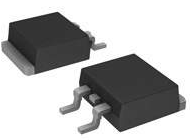
\includegraphics[width=0.4\linewidth]{Figures/Schottky_diode.PNG}}
	    \subfigure[Schottky diode pinout.]{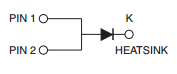
\includegraphics[width=0.4\linewidth]{Figures/Schottky_diode_pinout.PNG}}
	  \end{subfigmatrix}
	  \caption{Schottky diode VBT3045BP-E3 and pinout of the device.}
	  \label{fig:Schottky diode VBT3045BP-E3}
	\end{figure}
\end{center}